\chapter{Background}
\label{ch:background}

\section[\texorpdfstring{\msp}{MSP430}]{MSP430}

\msp is a family of low-power microcontrollers produced by Texas Instruments. The \msp ISA was chosen to be the target of the verification effort of this thesis for two reasons. Firstly, some models (\msp[FR58xx], \msp[FR59xx], \msp[FR6xx]) implement \intro{Intellectual Property Encapsulation}[IPE], a basic form of TEE; this means that there are meaningful security properties to be verified. Additionally, \msp microcontrollers are widely used in commercial applications, so they serve as a case study for the applicability of Katamaran to real-world architectures.

In short, IPE protects a user-defined memory region from being accessed by untrusted code. Assuming that the attacker can execute arbitrary code on the microcontroller, IPE is meant to:
\begin{itemize}
\item protect proprietary code from being leaked;
\item prevent the attacker from reading cryptographic keys and other sensitive data stored in memory;
\item maintain integrity of the protected region, so that code cannot be tampered with to produce leaks.
\end{itemize}

\msp microcontrollers include multiple additional hardware and software security features, such as limiting JTAG access, protecting the bootcode with a password \cite{slaa685} and a \intro{Memory Protection Unit}[MPU]. We will focus on IPE for the rest of the thesis.

\subsection{General characteristics}

The \msp has a 16-bit architecture, with some models supporting a 20-bit address space via an extended instruction set.

The ISA doesn't have dedicated load and store operations, but includes a rich set of addressing modes that allow access to memory and can be used with almost all instructions. For example, \texttt{add @r4+, 2(r5)} adds the word stored at the address contained in register \reg{r4} to the word stored at the address contained in \reg{R5} plus two, stores the result in the latter location, and increments \reg{R4} by two; the indirect autoincrement mode is used for the source, the indexed mode for the destination.

A peculiarity of the \msp is the adoption of FRAM \cite{slaa628b} to support most of the address space, with limited use of SRAM. FRAM is non-volatile, meaning that writes persist across reboots and losses of power.

\subsection{IPE}
\label{sec:ipe}

We will now discuss the workings of IPE in more detail.

To protect a region of FRAM, the user writes the start and end addresses without the 4 least significant bits\footnote{To allow the use of IPE on models with a 20-bit address space (and 16-bit registers, as usual). These bits must also be dropped in 16-bit address space models for portability.} to two memory-mapped registers, \reg{MPUIPSEGB1} and \reg{MPUIPSEGB2}. Then, IPE must be enabled by setting bit 6 (\regbit{MPUIPENA}) of the \reg{MPUIPC0} control register.

As long as \regbit{MPUIPENA} is set, read and write accesses to addresses contained in the protected region are only allowed if the program counter is also within the region, \ie the IPE range determines both the protected data and the trusted/privileged code.

There are some exceptions to this rule:
\begin{itemize}
\item the \intro{Interrupt Vector Table}[IVT] is always readable and writable, even if it overlaps with the IPE region; % actually depends on MPU too, also IVT under IPE is not executable (the IVT contains only pointers to interrupt routines anyway)
\item code executed from the first 8 bytes of the IPE range does \emph{not} have permission to access the protected region---the motivation will be explained in the next section.
\end{itemize}

If a violation occurs the microcontroller performs either a non-maskable interrupt or a \intro{power-up clear} (a type of device reset), depending on bit 5 (\regbit{MPUIPVS}) of \reg{MPUIPC0}.

After the IPE registers are configured, bit 7 (\regbit{MPUIPLOCK}) of \reg{MPUIPC0} can be set to prevent their further modification. They will not be allowed to change (triggering an IPE violation if a write is attempted) until a \intro{brown-out reset}[BOR] happens.
% Unlike PUCs, BORs do not clear the memory;
% Since most of the address space is comprised of non-volatile FRAM,
Untrusted code can disable the protections by causing a BOR and unsetting \regbit{MPUIPENA}, thus IPE configuration and locking should happen before the execution of application code, \ie in the bootcode.

\subsection{IPE initialization via bootcode}
\label{sec:bootcode}

The bootcode shipped with the \msp microcontrollers can read an IPE configuration from memory and apply it before any user code is executed.  It proceeds as follows:
\begin{enumerate}
\item Checks whether the user enabled this feature by writing \hex{AAAA} to location \addr{FF88} (\intro{IPE Signature 1}). If not, skips the following steps.
\item Reads the \intro{IPE structure pointer}[ISP] from location \addr{FF8A} (\intro{IPE Signature 2}). The user should have written the IPE configuration to the memory pointed to by the ISP, in the following format: three words for the values of \reg{MPUIPC0}, \reg{MPUIPSEGB2}, \reg{MPUIPSEGB1}; a word-size check code (odd bit-interleaved parity).
\item Stores the ISP in protected non-volatile memory.
\item Computes parity of the IPE structure to detect corruption. Initiates a full erase of memory if the computed parity isn't consistent with the check code, minimizing the likelihood of memory corruption causing exposure of protected data.
\item Configures the IPE registers according to the structure.
\end{enumerate}

Since the IPE Signature may not be protected by IPE, reading it at each boot lets the attacker change the IPE settings by overwriting the signature and rebooting. Therefore, on subsequent execution (recognized by the fact that the saved ISP is not null) the IPE Signature is not read. Regardless of its value, the structure pointed to by the saved ISP is checked for parity and used to initialize the registers.  To revert to the first-boot behavior, a special full-erase sequence must be performed through the JTAG interface.

The user can freely choose the location of the IPE structure, but is expected to place it within the IPE boundaries---particularly in the first 8 bytes, that are protected but not considered trusted code---to prevent it from being overwritten by attacker code. Overall, this affords trusted code the flexibility to change the protected range across reboots (which would not be possible if locking was truly permanent) securely.

\subsection{Security}
\label{sec:ipe-attacks}

As demonstrated by \cite{Bognar2024}, current implementations of IPE are vulnerable to a number of attacks, both architectural and via side-channels. These attacks assume an attacker that can execute arbitrary untrusted code (\ie can manipulate freely unprotected memory), which is a common threat model in discussions about TEEs.

Given our verification goal, of particular interest to us are the architectural attacks, which arise from inconsistencies in the ISA specification or errors in its hardware implementation. We briefly cover some of the vulnerabilities belonging to this class.

\subsubsection{Controlled call corruption}
\label{sec:call-corruption}

The \msp architecture provides a \asm{call} \emph{dst} instruction that saves the current \intro{program counter}[PC] to the stack, whose top element is pointed to by the \reg{SP} register, and jumps to \emph{dst}. IPE's permission checks are implemented erroneously for this instruction, opening the way for an attack (\cref{lst:call-corruption}):
\begin{lstlisting}[
  language=asm,
  float=htb, label=lst:call-corruption,
  caption={Attacker code for controlled call corruption.}
]
  mov #protected, SP
  call #ipefunc
\end{lstlisting}
\begin{enumerate}
\item an address (\asm{protected}) contained in the IPE region is written to \reg{SP}, which can be manipulated like a general purpose register;
\item a \asm{call} is performed to a trusted function (\ie to an address \asm{ipefunc} within the IPE boundaries).
\end{enumerate}

The \asm{call} instruction then attempts to write the return address (current PC) to the stack. The operation should fail, since the \reg{SP} is now in the IPE region and the \asm{call} is performed from untrusted code. Instead, on current models the write goes through successfully; it seems that the program counter is updated \emph{before} performing the access permission check.

This attack grants untrusted code the ability to corrupt protected memory. The values that the attacker can choose to write are restricted to those that are memory addresses from which the \asm{call} can be executed. Still, being able to write a known value is often sufficient to accomplish the attacker's goal (\eg replacing an encryption key), and the writable values include the encoding of many instructions. With enough effort the attacker is likely to be able to dump the whole content of the IPE region; controlled call corruption can break confidentiality as well as integrity of secured data and code.

\subsubsection{Code reuse}
\label{sec:code-reuse}

The IPE region doesn't have well-defined entry points; jumping to arbitrary protected locations is always allowed. This opens the door to code reuse attacks. As an example, \cref{lst:read-gadget} shows a piece of trusted code that copies a word from memory location \asm{src}  to \asm{dst}. For the attacker, it easily becomes a universal read and write gadget: it is sufficient to write the desired source and destination addresses to \reg{r4} and \reg{r5}, and then jump directly to the third line.

\begin{lstlisting}[
  language=asm,
  float=htb, label=lst:read-gadget,
  caption={An innocuous copy can become a universal read gadget.}
]
  mov #src, r4
  mov #dst, r5
  mov 0(r4), 0(r5)
\end{lstlisting}

In isolation, performing this attack is not trivial, since the IPE code is confidential; identifying suitable gadgets may require a lot of trial and error. Other attacks (including side-channel attacks) may be used to aid this search, and finding a universal write gadget turns a vulnerability that breaks confidentiality into one that also breaks integrity.

\subsubsection{Interrupting IPE code}
\label{sec:interrupts}

Interrupts are handled as usual during execution of protected code: the processor consults the interrupt vector table to find the location of the appropriate \intro{interrupt service routine}[ISR], and execution continues from there, until the routine returns to the code that was interrupted. It is the responsibility of the ISR to restore the general purpose registers to their initial value before returning.

The IVT is always writable, even when inside the IPE boundaries. The attacker can configure an ISR, call a trusted function and interrupt it; the ISR can then:
\begin{itemize}
\item examine the contents of the registers used by the trusted code;
\item modify them, altering the trusted code's behavior.
\end{itemize}

One official document \cite{slaa685} suggests disabling interrupts during execution of IPE code to avoid this issue. However, there is no way to disable non-maskable interrupts, and the lack of well-defined entry points allows the attacker to jump over the code that disables the maskable interrupts.

\section{Formal specification of ISAs}
\label{sec:formal-isa}

Major hardware vendors specify their architectures with varying degrees of detail and precision. Intel's \cite{Intel2025} and AMD's \cite{AMD2024} x86 manuals are mostly prose, with some pseudocode to aid understanding. Power's specification \cite{OPF2024} is accompanied by comprehensive pseudocode, for which a parser has been developed \cite{libreSOC}. Armv8's semantics is specified precisely using the ASL language \cite{Arm2020}\cite{Reid2016}; the same goes for RISC-V with the Sail language \cite{RVSail}.

Compared to natural-language manuals, formal machine-readable specifications define exactly the behavior of the architecture without room for ambiguity, and they provide a base for formal (automated) reasoning \cite{Armstrong2018}.

Texas Instruments does not provide an official formal specification for the \msp microcontrollers. We base our verification work on an extension of the \msp Sail model developed in \cite{mspthesis}.

\subsection{Structure of a Sail specification}
\label{sec:sail-structure}

Sail \cite{Armstrong} is a language designed for the purpose of specifying ISAs. Its tooling can generate emulators (by translation to C or OCaml) and definitions for theorem provers (\eg Rocq and Lem) to reason about the ISA.

Sail specifications are typically interpreters of the target architecture's machine code. The main function runs a fetch-decode-execute cycle that mirrors that of the hardware:
\begin{labeling}[~--]{execute}
\item[fetch] read from memory the word pointed to by the \reg{PC} register;
\item[decode] parse the result of fetch (a bitvector) into a structured representation;
\item[execute] pattern match on the instruction to perform the appropriate side effects, such as modifying registers or writing to memory.
\end{labeling}

This style facilitates extraction of executable code from the ISA and the development of the specification by engineers without further training, as opposed to \eg custom small-step semantics.

Sail code doesn't usually concern itself with the details of memory. Instead, it is common to declare functions like \sail{read_ram} and \sail{write_ram} as foreign, \ie implemented in a language other than Sail. When extracting an emulator a concrete implementation must be given in C or OCaml.

\subsection{The Sail language}

At its core, Sail is a first-order imperative language that integrates a number of features commonly found in vendor-specific pseudocode and specification languages. The result is an expressive set of primitives that ease both manual development of new specifications and automated translations from the pseudocode languages that inspired Sail.

This section outlines some of Sail's distinctive features.

\begin{figure}
  \centering
  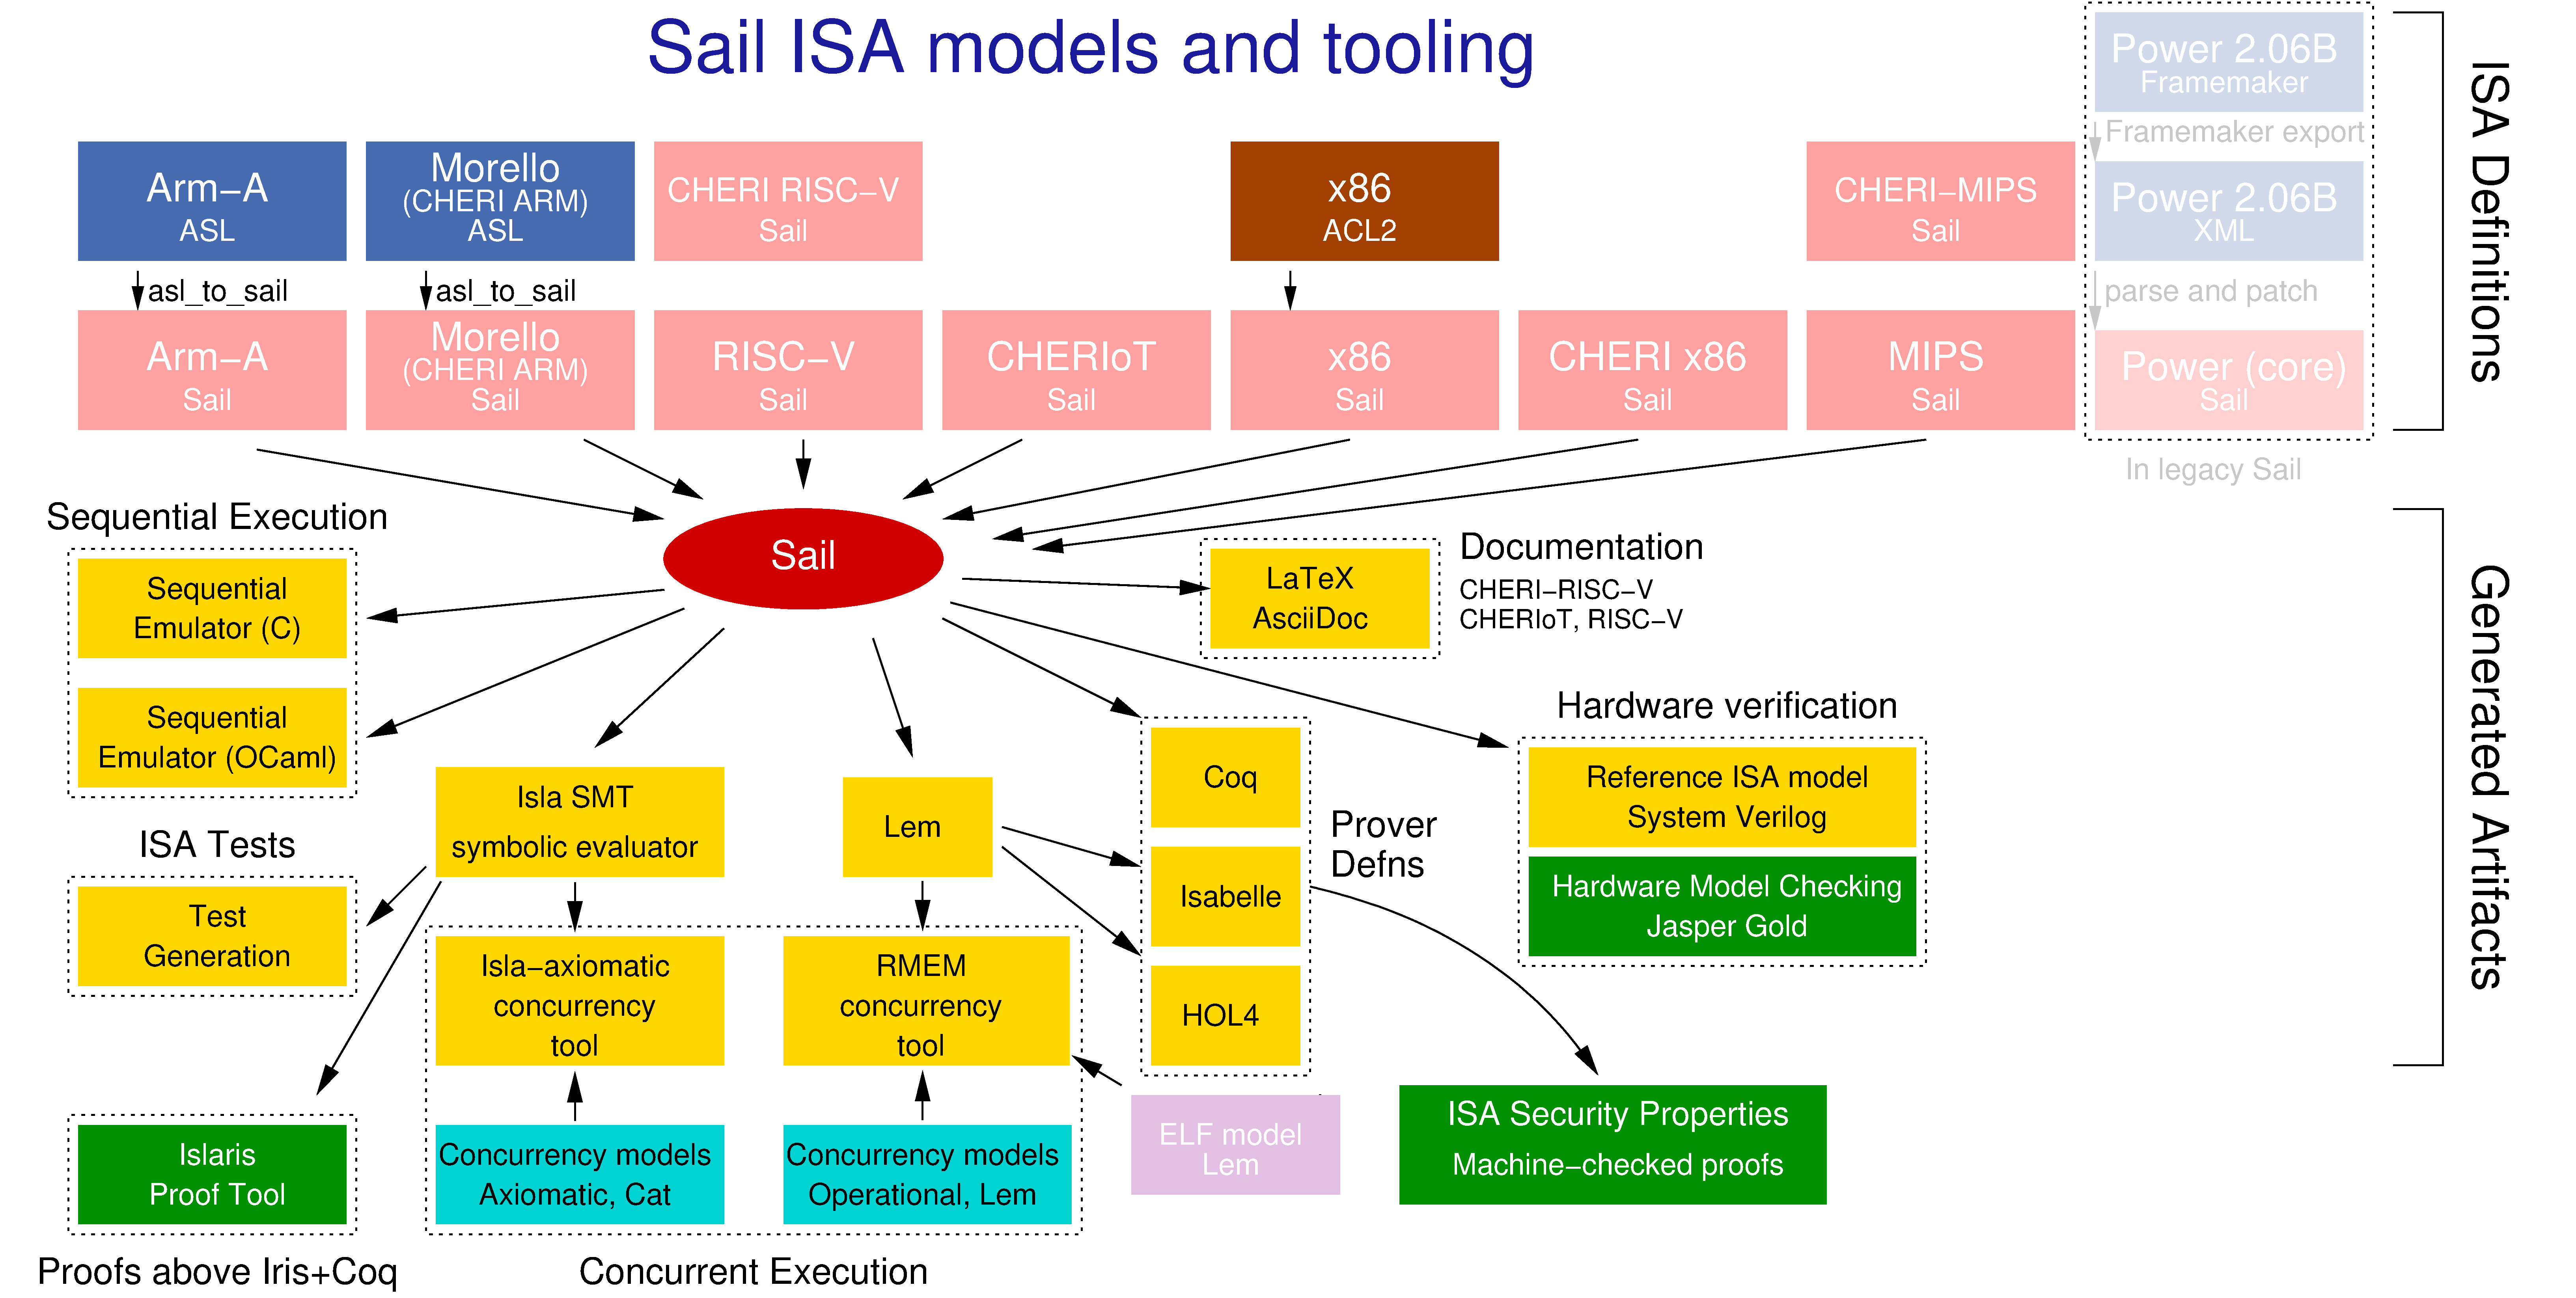
\includegraphics[width=12cm]{sail-overview}
  \caption{Overview of the Sail infrastructure (from Sail's GitHub repository).}
  \label{fig:sail-overview}
\end{figure}

\subsubsection{Expressive types}

Sail's type system supports user-defined structs, enums and unions (sum types).

The built-in types include arbitrary-precision integers (\sail{nat} and \sail{int}), bounded integers (\eg \sail{range(0, 15)}) and bitvectors of a given length (\eg \sail{bits(8)}).

A limited form of dependent types is available, primarily to rule out the possibility of out-of-bounds accesses to bitvectors. In Sail, types can be of three kinds: \sail{Type}, the kind of enums, structs, \sail{nat}, \sail{bvec(n)}, etc.; \sail{Int}, the kind of integers; \sail{Bool}, of \sail{true} and \sail{false}.

Consequently, integers can be used in types (as seen in \eg \sail{bits(8)}), and polymorphic type variables can range over integers, as they are themselves types.

As an example, a function that repeats a bitvector some number of times could have the following signature:

\begin{lstlisting}[language=sail]
  val replicate_bits : forall 'n 'm, 'm >= 1 & 'n >= 1.
      (int('n), bits('m)) -> bits('n * 'm)
\end{lstlisting}

\sail{replicate_bits}'s type is parameterized over two type variables \sail{n} and \sail{m}, which are inferred to be of kind \sail{Int}; at each usage site they will be instantiated with some integer. Next we set two constraints for the integer type variables: they must be at least 1. Finally, we state that \sail{replicate_bits} is a function with:
\begin{description}
\item[Inputs] an integer and a bitvector. At each call site, the type variable \sail{n} will be instantiated with the integer, and \sail{m} with the size of the bitvector.
\item[Output] a bitvector of size \(\sail{n} \cdot \sail{m}\).
\end{description}
So the return type of \sail{replicate_bits(4, 0b0101)} is \sail{bits(16)}.

Dependent types can be eliminated through monomorphization when exporting to a target that doesn't support them, such as Lem and Isabelle/HOL.

% type variables can be used in expressions but non freca

\subsubsection{Pattern matching}

Pattern matching is a pervasive operation in all kind of interpreters, and machine code specifications are no exception. Sail's patterns can be used to match and destruct structs, tuples, unions, enums, bitvectors and more. As usual, patterns double as l-values when they are irrefutable.

Bitvector patterns are a distinctive feature that comes from existing pseudocode conventions. For instance, the following pattern matches the encoding of the RISC-V \texttt{ADDI} instruction:
\begin{lstlisting}[language=sail]
  imm : bits(12) @ rs1 : bits(5) @ 0b000 @ rd : bits(5) @ 0b0010011
\end{lstlisting}
it will bind the first 12 bits to \sail{imm}, the following 5 to \sail{rs1}, then expect 3 zeroes, followed by 5 bits bound to \sail{rd}, and then the sequence \texttt{0010011}.

\subsubsection{Scattered definitions}

A single union, enum or function can have its definition split between multiple locations, possibly in different files. A common use case is to partition decoding and execution by instruction.

\begin{lstlisting}[language=sail]
  union clause ast = ADDI : (bits(12), regbits, regbits)

  function clause decode(imm : bits(12)
                         @ rs1 : regbits @ 0b000
                         @ rd : regbits @ 0b0010011)
    = ADDI(imm, rs1, rd)

  function clause execute (ADDI(imm, rs1, rd)) = ...
\end{lstlisting}

\subsubsection{Overloading}

Sail supports function and operator overloading, as found \eg in ASL \cite{Reid2016}. A common pattern consists in defining two functions \sail{read(reg)} and \sail{write(reg, v)}, and then an overload \sail{overload X = \{read, write\}}, to be used as in \sail{X(R5) = X(R4) + 0x0001}.

\section{Security properties as universal contracts}
\label{sec:universal-contracts}

Once we have a precise account of our architecture's semantics, we likewise need a formal way of expressing security guarantees. Our language of choice for doing so is separation logic.

\subsection{Security contracts}

The basic idea is to verify contracts, or Hoare triples, that encode security properties. Take for example the security property: ``a closed door cannot be
unlocked without providing the password 123''. It is encoded by the following contract:
\[ \hoare
  {\text{door locked} \wedge \mathit{pwd} \neq 123}
  {\texttt{unlock-door(\(\mathit{pwd}\))}}
  {\text{door locked}} \]

The contract states that for all values of \(\mathit{pwd}\), if the precondition (\(\text{door locked} \wedge \mathit{pwd} \neq 123\)) holds and we execute \(\texttt{unlock-door(\(\mathit{pwd})\)}\), then the postcondition (door locked) will hold after that.

Note that we are not saying anything about what \texttt{unlock-door} \emph{does}, \ie its functional specification or axiomatic semantics. Rather, our properties constrain the abilities of an attacker (in this case of opening the door without knowing the password), so they mostly tell us what the function \emph{doesn't} do.

\subsection{Universal contracts}

Knowing \texttt{unlock-door}'s implementation, we can prove that the above contract holds. We could verify similar security properties for all functions in a program. This technique is applicable whenever:
\begin{itemize}
\item we are only dealing with known (trusted) code, or
\item the attacker can only interact with our program/machine by calling known functions.
\end{itemize}

Given our threat model, neither of the above assumptions holds true. We want to ensure that the guarantees hold when executing attacker code, which cannot be known a priori. We deal with this by proving the security property for \emph{all} programs, encompassing all possible attacker behaviors:
\[ \forall p.\; \hoare{\text{assumptions}}{p}{\text{security guarantees}} \]
this is known as a \emph{universal contract}.

For an example relevant to the \msp, we could wish to express the property that locked IPE registers cannot be modified (\(p\), like all free variables, is implicitly universally quantified):
\[ \hoare
  {c = \text{current IPE config} \wedge c.\mathrm{locked}}
  {p}
  {c = \text{current IPE config}} \]

\subsection{Contracts on the Sail specification}

In the above contract \(p\) is a \msp machine program. Its proof would be conducted on the semantics of the \msp ISA, which we derive from its Sail specification: the semantics of a machine code instruction is the result of evaluating the \sail{decode} and \sail{execute} functions on that instruction. We can make this explicit in our contracts:
\[ \hoarem
  {\begin{aligned}
    &\text{memory contains \(p\) starting from PC} \\
    &{}\wedge c = \text{current IPE config} \wedge c.\mathrm{locked}
  \end{aligned}}
  {\texttt{fdeCycle()}}
  {c = \text{current IPE config}} \]

ISAs' security guarantees can be usually reduced to properties that hold after executing single instructions. Here, if after executing any single instruction the IPE registers are unchanged, it follows that any sequence of instructions (\ie arbitrary program) also leaves them unchanged.\footnote{This kind of reasoning is sound when the postcondition of every instruction in the sequence implies the precondition of the next, which is true here: if the configuration is locked at the beginning of \sail{execute} and it unchanged at the end, it is also locked at the end, so we can apply again the contract to the next instruction.} We can thus give a simpler (to express and verify) contract on just the execute step of the fetch-decode-execute cycle:
\[ \hoare
  {c = \text{current IPE config} \wedge c.\mathrm{locked}}
  {\texttt{execute(\(\mathit{instr}\))}}
  {c = \text{current IPE config}} \]

% Repeated application of this contract for the verification of multi-instruction programs is justified by the fact that the postcondition implies the precondition.

% Here the reduction to the single instruction case is justified by the fact that the postcondition implies the precondition: after executing any instruction under the assumption that the configuration is locked we know that the configuration is still locked, therefore we can apply the contract to the next instruction and so on.

The shift in viewpoint from assembly to Sail code is consequential for machine-assisted proofs of security contracts. Verification tools need only know about the semantics of the Sail language, which remains fixed, and can be agnostic about the details of the ISAs they are applied to.

\subsection{Separation logic}

So far we have been stating the pre- and postconditions informally. To make them more precise we need a language that can express properties involving memory, registers and access permissions, while being simple enough to facilitate (semi-)automated reasoning. The obvious choice here is a basic separation logic.

Generally speaking, separation logic is a kind of Hoare logic extended with predicates that state ownership of \emph{resources}, such as memory locations and registers. For example, \(\ell \ptom v\) (pronounced \(\ell\) points to \(v\)) asserts that we own the location \(\ell\) and that the value stored at that location is \(v\).

Separation logic introduces a new connective, the \intro{separating conjunction}. \(P \ast Q\) (\(P\) and separately \(Q\)) is true when \(P\) and \(Q\) both hold and have exclusive ownership of the resources they assert. For example, while \(\ell \ptom v \wedge \ell \ptom v\) is true for a memory where location \(\ell\) stores \(v\), \(\ell \ptom v \ast \ell \ptom v\) is always false, as the two conjuncts don't have exclusive ownership of \(\ell\). So from the validity of \(\ell_1 \ptom v \ast \ell_2 \ptom v\) we can derive that \(\ell_1 \neq \ell_2\).

The point of this is to enable modular reasoning in the presence of mutable state. Separation logic's proof system has a key rule in this regard:
\[ \frac{\hoare{P}{e}{Q}}{\hoare{P \ast R}{e}{Q \ast R}}[\textsc{Frame}] \]
Intuitively, from the premise we learn that \(e\) only requires the resources described by \(P\) to produce \(Q\); from that we deduce that it doesn't alter the resources described by \(R\). The frame rule doesn't hold for \(\wedge\), otherwise from \(\hoare{\ell \ptom 0}{\ell \leftarrow 1}{\ell \ptom 1}\) we could deduce \(\hoare{\ell \ptom 0 \wedge \ell \ptom 0}{\ell \leftarrow 1}{\ell \ptom 1 \wedge \ell \ptom 0}\), which is unsound; separating conjunction is not affected because it ensures exclusiveness of ownership.

There is also another new connective, the \intro{magic wand}, written \(P \wand Q\). It is to the separating conjunction what implication is to logical conjunction; it means that we have the resource \(Q\) if we satisfy \(P\).

The postcondition of a triple can refer to the value returned by the expression with the notation \(\hoare{P}{e}[v]{Q}\). We consider the triple to hold also when \(e\) doesn't terminate or throws an exception, irrespective of the validity of \(Q\).

\subsection{Memory access permissions with separation logic}
\label{sec:sep-logic-permissions}

It is possible to use separation logic to express the property that a piece of code only has access to a limited region of memory.

For that, we assume the following specifications for \texttt{read\_ram} and \texttt{write\_ram}:
\begin{gather*}
  \hoare{\ell \ptom v}{\texttt{write\_ram($\ell$, $v'$)}}{\ell \ptom v'} \\
  \hoare{\ell \ptom v}{\texttt{read\_ram($\ell$)}}[u]{u = v \wedge \ell \ptom v}
\end{gather*}
we are only ``allowed'' to access a location if we own the corresponding chunk of memory. Concretely, we cannot prove any triple\footnote{Excluding those with an inconsistent precondition.} for a program that reads or writes to memory unless we assume the appropriate points-to predicates in the precondition.

So if we want to state that the \coq{store} instruction doesn't let the attacker write to protected memory, we do that with the triple:
\[ \hoare{\bigast_{\smash{\mathrm{unprotected}~\ell}} \exists v.\; \ell \ptom v}{\texttt{execute\_store($l$, $u$)}}{\top}\]
Since the precondition doesn't include points-to chunks for protected locations, the contract is provable only if \texttt{execute\_store} never attempts to access them, regardless of whether its argument \(l\) is protected.

Thus the implementation \texttt{execute\_store(\(l\), \(u\)) = write\_ram(\(l\), \(u\))} wouldn't satisfy the contract: there is no way to prove any postcondition, not even the trivial one, because \texttt{write\_ram}'s specification requires ownership of \(l\), which we don't have in general.

On the other hand,
\begin{lstlisting}[language=sail, mathescape]
  function execute_store($l$, $u$) =
    if protected $l$ then throw error()
    else write_ram($l$, $u$)
\end{lstlisting}
only invokes \texttt{write\_ram} when we know that \(l\) is unprotected, and thus can prove that we own its chunk. We are able to apply \texttt{write\_ram}'s specification and derive a postcondition about \texttt{execute\_store}, therefore proving the contract. Provability coincides with the implementation being safe, \ie not allowing forbidden accesses at runtime.

\section{Katamaran}
\label{sec:katamaran}

Katamaran \cite{Huyghebaert2023} is a framework for the semi-automated verification of ISAs. It is built on top of the Rocq\footnote{Until recently known as Coq.} theorem prover and the Iris separation logic framework.

\begin{figure}[htb]
  \centering
  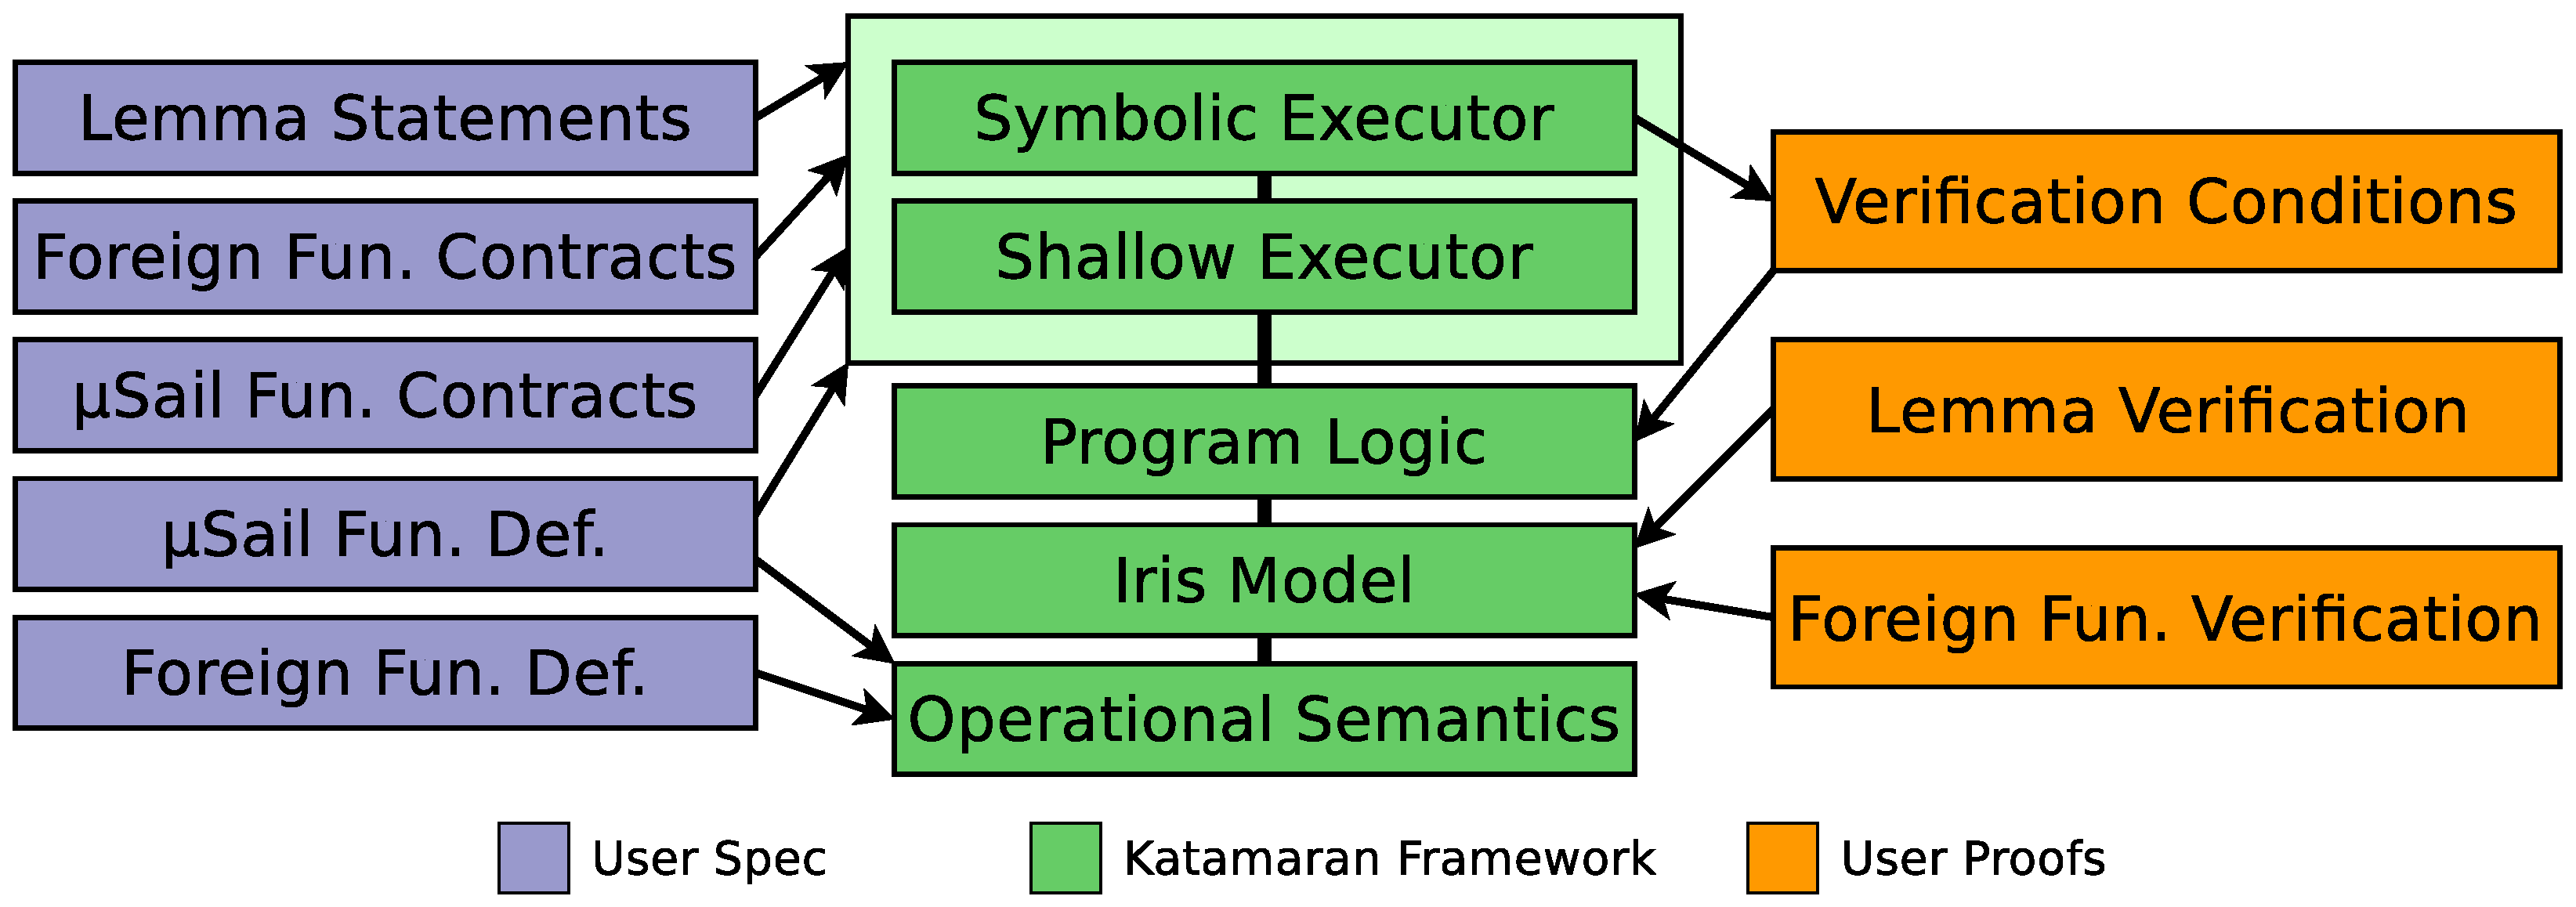
\includegraphics[width=12cm]{katamaran.eps}
  \caption{Katamaran's architecture (from \cite{Huyghebaert2023})}
  \label{fig:katamaran}
\end{figure}

\Cref{fig:katamaran} shows the components of a mechanized proof based on Katamaran. Firstly, the user needs to provide a \usail (a subset of Sail embedded in Rocq) model of the ISA and the contracts they want to prove. Katamaran's symbolic executor then runs the object code of the contracts under the given preconditions and checks that the postconditions match. If it cannot prove that they do or don't, it leaves some \intro{verification conditions}[VCs] that the user can inspect and verify manually using Rocq's tactic language.

The symbolic executor can only reason about \usail code. For all foreign functions used in the model a specification must be provided. Whenever the foreign function is called, its contract will be applied to determine the effects of the call.

Pre- and postconditions are specified in a simple separation logic that can be extended with user-defined resources. These resources are opaque to the solvers and must be manipulated explicitly by invoking user-provided lemmas, which are essentially contracts that apply to the empty program.

The result of this process is the guarantee that the verified contracts hold up to the validity of the foreign function contracts and lemmas. Lemma correctness can be then proved by instantiating Katamaran's Iris model with a definition of the custom resources in terms of Iris propositions, and carrying out the proof via Iris' tactics. Likewise, foreign function contracts can be verified against a Rocq implementation of those functions. After that we have full assurance that the ISA satisfies the desired properties, as Katamaran itself is also proved correct.

